\subsection{\label{subsec:FZV2}Franck-Condon Prinzip}
\textbf{\textit{Erläutern Sie das Franck-Condon Prinzip.}} \\
$\rightarrow$
Im Folgenden leiten wir den Franck-Condon Faktor und das damit verbundene Prinzip
schematisch her. \\
Sieht man das einfallende elektromagnetische Feld des Anregungslichtes als
Störung, so kann man mithilfe des Dipol-Operators $\hat{\mu}$ und
Fermis Goldener Regel die Übergangswahrscheinlichkeit eines elektronischen
Übergangs vom Zustand $i$ nach $f$ bestimmen. \newpage
Hierfür wird das bereits
in vorheriger Frage erwähnte Übergangsdipolmoment $D_{if}$ benötigt, welches sich
folgendermaßen ergibt
\begin{equation}\label{eq:deflangle}
    D_{if} = \langle\Psi_{i}\vert \hat{\mu} \vert \Psi_{f}\rangle = \int\int\,d\mathbf{r}^{N_{\text{Elektron}}}\,d\mathbf{R}^{N_{\text{Kern}}} \Psi_{i}^{*}\hat{\mu}\Psi_{f},
\end{equation}
wobei $\Psi$ die von $\mathbf{R}$ und $\mathbf{r}$ also Kern- und Elektronenkoordinaten abhängigen Gesamtwellenfunktionen
der jeweiligen Zustände sind. \\
Nach der Born-Oppenheimer Näherung kann die Zustandswellenfunktion des Moleküls in einen Anteil der
Elektronen und einen Anteil der Kerne wie folgt aufgeteilt werden
\begin{equation}
    \Psi_{\text{Molekül}}(\mathbf{r}^{N_{\text{Elektron}}}, \mathbf{R}^{N_{\text{Kern}}}) \approx \chi_{\text{Kern}}(\mathbf{R}^{N_{\text{Kern}}})\,\phi_{\text{Elektron}}(\mathbf{r}^{N_{\text{Elektron}}}, \mathbf{R}^{N_{\text{Kern}}}).
\end{equation}
Diese Näherung ist möglich und sinnvoll, da die Atomkerne sehr viel schwerer als die Elektronen sind und daher quasi stillstehen. \\
Für die Herleitung des Franck-Condon Faktors wird diese Argumentation übernommen und man nimmt an, dass die elektronischen
Übergänge sehr viel schneller stattfinden als die Kerne der Bewegung folgen können. Der Übergang wird folglich
in zwei Schritte aufgeteilt, wonach sich im ersten Schritt die Elektronenwellenfunktion instantan ändert
und hiernach die Kernposition angepasst wird. Für die Berechnung folgt daher, dass die Kernposition
$\mathbf{R}$ in der Elektronenwellenfunktion nur mehr ein Parameter und keine Variable mehr ist. \\
Teilt man zusätzlich den Dipol-Operator durch die Position der positiven und negativen Ladungsträger auf,
so folgt
\begin{align}
    \hat{\mu}          & = \hat{\mu}_{\text{E}} + \hat{\mu}_{\text{K}}                                                          \\
                       & = -e\mathbf{r}^{N_{\text{E}}} + q_{\text{K}}\mathbf{R}^{N_{\text{K}}}                                  \\
    \Rightarrow D_{if} & = \langle\chi_{i}\psi_{i}\vert \hat{\mu}_{\text{E}} \vert\chi_{f}\psi_{f}\rangle +
    \langle\chi_{i}\psi_{i}\vert \hat{\mu}_{\text{K}} \vert\chi_{f}\psi_{f}\rangle                                              \\
                       & = \langle\chi_{i}\vert \chi_{f}\rangle \langle \psi_{i}\vert \hat{\mu}_{\text{E}}\vert\psi_{f}\rangle.
\end{align}
Im letzten Schritt wurden die Integrale aufgeteilt, da $\mathbf{R}$ nur ein Parameter der Elektronenwellenfunktion
darstellt und der Beitrag über das Kern-Dipolmoment verschwindet, da die Elektronenwellenfunktionen
orthogonal zueinander stehen und damit das Integral zwischen zwei unterschiedlichen Zuständen verschwindet. \\
Der resultierende Vorfaktor $\langle\chi_{i}\vert \chi_{f}\rangle$ wird Franck-Condon Faktor genannt,
wobei dessen Betragsquadrat proportional zur Übergangswahrscheinlichkeit und damit zur Strahlungsintensität
des betrachteten Übergangs ist. \\
Nach Gl.~\eqref{eq:deflangle} gibt der Faktor Auskunft über die räumliche Überlappung zweier Kern-Schwingungs-Wellenfunktionen
und besagt, dass der Übergang für gute Überlagerung wahrscheinlicher ist. \\
Zusammengefasst beschreibt das Franck-Condon Prinzip den Umstand, dass elektronische (schwingungs-)Übergänge
wahrscheinlicher sind, wenn die Wellenfunktionen der Kerne räumlich stärker überlappen. Das Prinzip erscheint sinnvoll,
da die Elektronenbewegung deutlich schneller abläuft und daher ein senkrechter Übergang nur stattfinden kann,
wenn sich am betrachteten Ort ein Atomkern befinden kann. Diese Aufenthaltswahrscheinlichkeit wird über den
Franck-Condon Faktor berechnet \cite{EPC,Demtroder,Parson}. Das Prinzip ist in Abb.~\ref{fig:fcf} skizzenhaft
dargestellt. Der Übergang eines Vibrationszustandes im elektronischen Grundzustand $\text{v''}$ in einen elektronisch
angeregten Zustand ist senkrecht, da die Kerne der Elektronenbewegung nicht instantan folgen können. Der
wahrscheinlichste Übergang ist dieser, für den der Franck-Condon Faktor maximal wird und folglich die
Schwingungswellenfunktion der Kerne am stärksten überlappt ($\text{v''}=0 \rightarrow \text{v'}=2$).
Für die Relaxation in den Grundzustand findet dieses Prinzip erneut Anwendung.
\begin{figure}[h!]
    \centering
    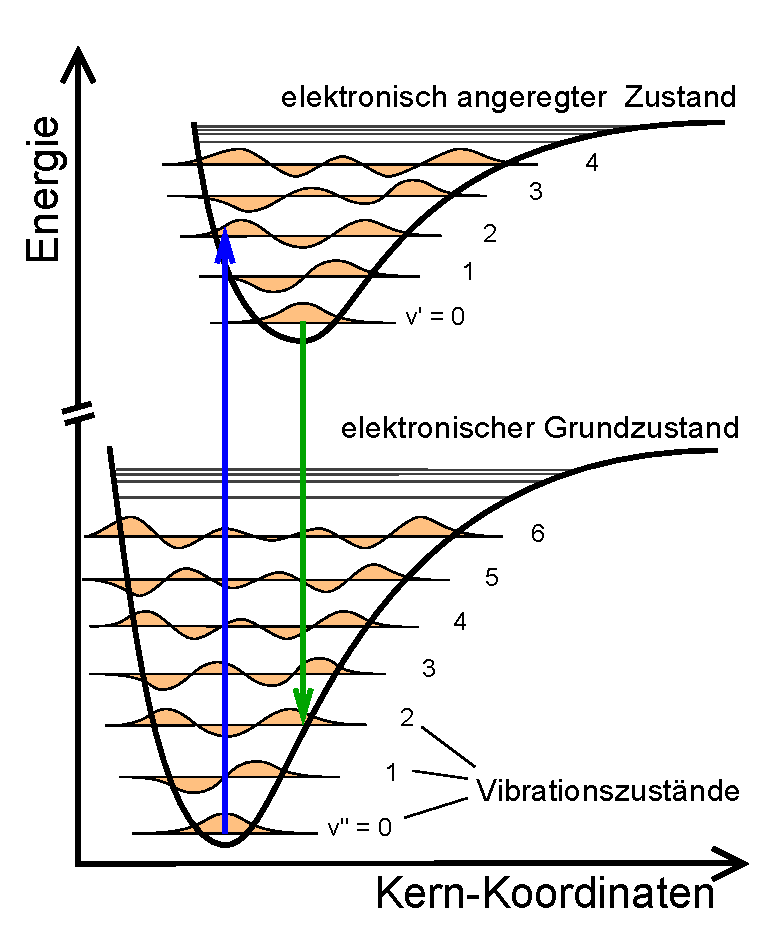
\includegraphics[width=0.4\textwidth]{fcf.pdf}
    \caption{\label{fig:fcf}Schematische Darstellung des Franck-Condon Prinzips. In einem elektronischen Zustand
        herrscht eine Potentiallandschaft (schwarz), die ihr Minimum bei der Gleichgewichtsposition der Kerne hat.
        Bei der Anregung in einen elektronischen Zustand verschiebt sich diese Gleichgewichtsposition und damit die
        Potentiallandschaft. Innerhalb der elektronischen Zustände gibt es unterschiedlich angeregte Schwingungszustände
        der Kerne (orangene Kurven). Eine große Übergangswahrscheinlichkeit, also ein großer Franck-Condon Faktor, ist für
        einen großen Überlapp dieser Schwingungszustände gegeben. Daher sind die eingezeichneten Übergänge (blau und grün)
        nach dem Franck-Condon Prinzip am wahrscheinlichsten. Die Grafik wurde Ref.~\cite{fcf} entnommen.}
\end{figure}\\ \FloatBarrier